
% Template for HC2 documents
% 
% Please create a different file for each language
%
% Dependencies:
% - This file should compile if you have installed all the LaTeX extensions
%   (texlive-full in Ubuntu)
% - You will need the program "hevea" to convert to HTML
%
% Caveats:
% - Please use the "verbatim" environment for code, and please use spaces instead of tabs
% - Hevea does not convert the images properly, however this can be done manually
%   (you just need to convert the pictures to PNG and rename your pictures  hc2template001.png
%   etc.) We will anyway have to do some magic with the HTML files so that they work
%   in Mooshak
% - Please use only $ and $$ for math environments, and never \begin{equation}
\documentclass[11pt,a4paper]{article}
\usepackage{mathptmx}
\usepackage[in]{fullpage}
\usepackage[absolute]{textpos}
\usepackage{graphicx}
\usepackage[frenchb]{babel}
\usepackage[utf8]{inputenc}
\usepackage[T1]{fontenc}
\usepackage{fancyhdr}
\usepackage{moreverb}
\usepackage{color}
\usepackage{url}
\usepackage{longtable}
\pagestyle{fancy}

\definecolor{gray}{RGB}{128,128,128}

\renewcommand{\baselinestretch}{0.92}

%%%%%%%%%%%%%%%%%%%%%%%%%%%%%%%%%%%%%%%%%%%%%%%%%%%%%%%%%%%%%%%%%%%%%%%%%%%%%%%%%%%%%%%%%

% Put the title of your document here
\newcommand{\titleinfolong}{Manuel d'équipe pour le Helvetic Coding Contest 2015}
\newcommand{\titleinfo}{Manuel d'équipe}
% Put the author of the document here
\newcommand{\authorinfo}{Robert R.~Enderlein}
% Put the language of the document here
\newcommand{\langinfo}{Français}
% Put the name of the Task (or some short identifying information of the document) here
\newcommand{\taskinfo}{Manuel}

%%%%%%%%%%%%%%%%%%%%%%%%%%%%%%%%%%%%%%%%%%%%%%%%%%%%%%%%%%%%%%%%%%%%%%%%%%%%%%%%%%%%%%%%%


\title{\titleinfolong}
\author{de \authorinfo\footnote{Ce document a été adapté à partir du manuel d'équipe de  Domjudge.}}
\date{}

\renewcommand{\headrulewidth}{0pt}
\renewcommand{\footrulewidth}{0.4pt}
\lhead{}
\chead{}
\rhead{}
\lfoot{\textcolor{gray}{Helvetic Coding Contest 2015}}
\cfoot{\thepage}
\rfoot{\textcolor{gray}{\titleinfo}}

\begin{document}
\maketitle
\thispagestyle{fancy}
\setcounter{page}{1} 

%\begin{latexonly}
\begin{textblock*}{20mm}(170mm, 15mm)

\includegraphics[width=20mm]{hc2logogray.pdf}
\end{textblock*}

\begin{textblock*}{50mm}(25.4mm, 25.4mm)
\noindent \textcolor{gray}{\langinfo \\ \textbf{\taskinfo} }
\end{textblock*}
%\end{latexonly}

%%%%%%%%%%%%%%%%%%%%%%%%%%%%%%%%%%%%%%%%%%%%%%%%%%%%%%%%%%%%%%%%%%%%%%%%%%%%%%%%%%%%%%%%%
%%%%%%%%%%%%%%%%%%%%%%%%%%%%%%%%%%%%%%%%%%%%%%%%%%%%%%%%%%%%%%%%%%%%%%%%%%%%%%%%%%%%%%%%%
%%%%%%%%%%%%%%%%%%%%%%%%%%%%%%%%%%%%%%%%%%%%%%%%%%%%%%%%%%%%%%%%%%%%%%%%%%%%%%%%%%%%%%%%%
% Start here

% There is a bug in the hevea package. The following construct will make sure
% that everything written in \heaveaonly will be written only in Hevea
% htmlonly doesn't work for some reason
\newcommand{\heveaonly}[1]{#1}
%\begin{latexonly}
\renewcommand{\heveaonly}[1]{}
%\end{latexonly}

\noindent Voici un bref résumé de la documentation du système. Il est conçu comme une introduction brève, afin que vous
puissiez commencer à utiliser le système rapidement. Nous conseillons fortement qu'au moins une personne dans votre équipe
lise le manuel dans son intégralité. Certains détails spécifiques
à ce système peuvent devenir importants si vous avez un problème.

Vous pouvez accéder à l'interface web de Domjudge depuis
\url{https://ec2.hc2.ch/team}.
Voir Figures \ref{fig:overview}, \ref{fig:statements}, \ref{fig:ranking}
pour un aperçu.

\paragraph{Énoncés des problèmes et documents de support.}
Les énoncés des problèmes et documents de support sont 
disponibles par le lien \og Problem statements\fg{} depuis votre page d'équipe.
Notez que certains problèmes sont grisés: vous ne serez pas
en mesure de voir les énoncés jusqu'à ce que vous avez
résolu le problème au dessus de celui-ci.
Voir Figure~\ref{fig:statements}.

\paragraph{Lecture et écriture.}
Votre solution devra lire la donnée depuis l'entrée
standard et écrire la réponse sur la sortie standard.
Vous ne devez pas ouvrir d'autre fichiers.
Voir Section~\ref{codeexamples} pour quelques exemples
de solutions. Utilisateurs de Java: nous vous déconseillons
l'utilisation de java.util.Scanner pour la lecture de
grosses données.

Java, Scala: prière de rester dans le paquet par défaut: n'utilisez pas la directive \texttt{package}.

\begin{figure*}[t]
\begin{center}
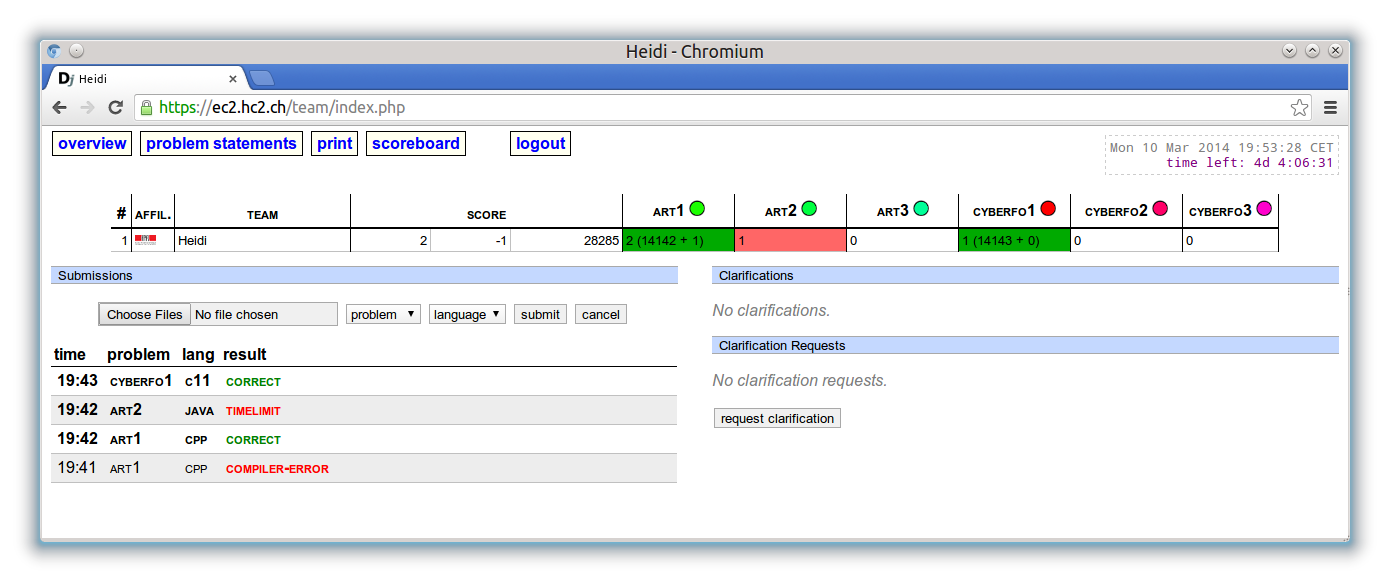
\includegraphics[width=0.73\textwidth]{overview.png}
\end{center}
\vskip -2 em
\caption{Page d'interface d'équipe.}
\label{fig:overview}

\begin{center}
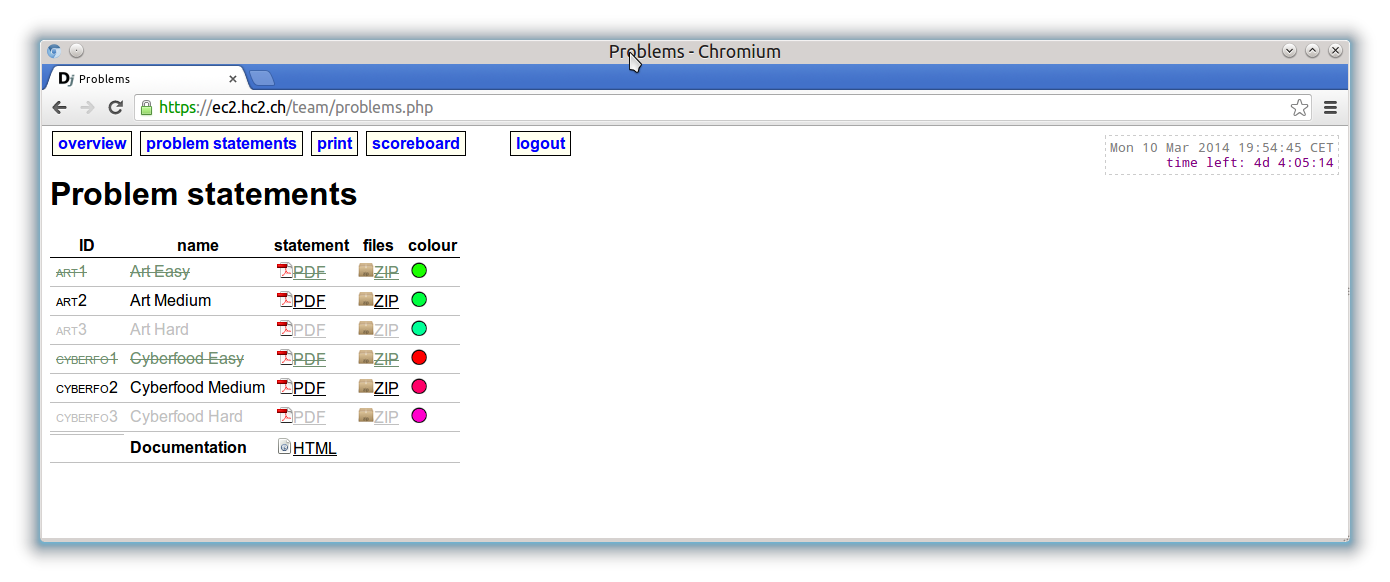
\includegraphics[width=0.73\textwidth]{statements.png}
\end{center}
\vskip -2 em
\caption{Page des énoncés des problèmes}
\label{fig:statements}

\begin{center}
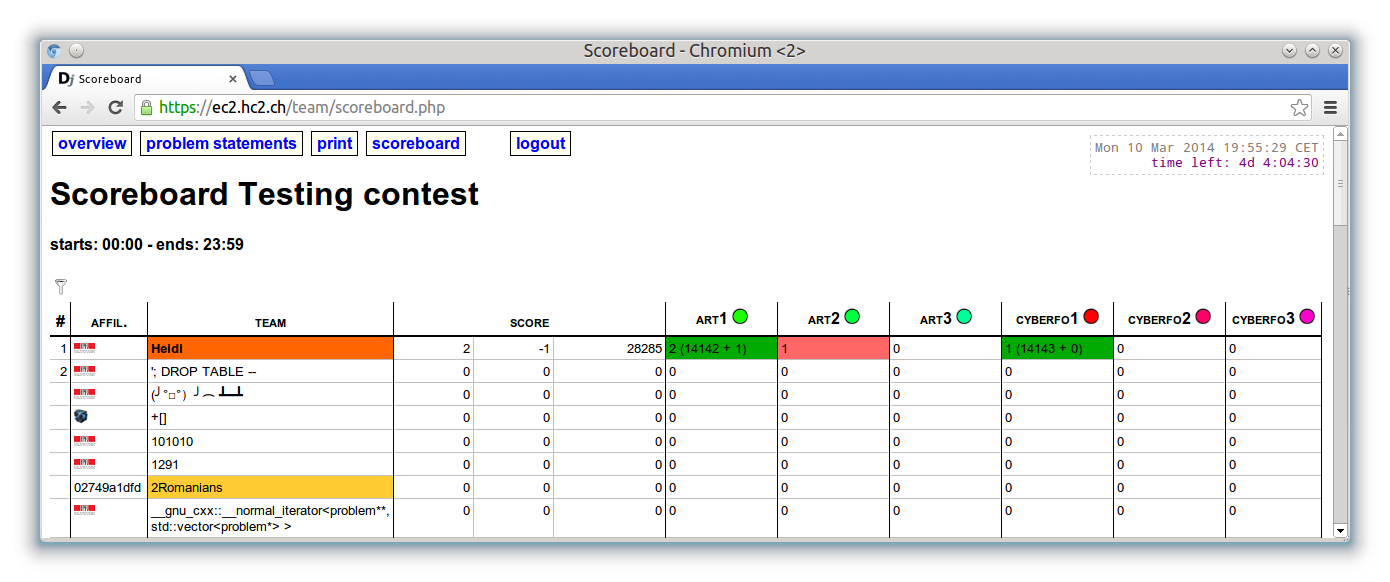
\includegraphics[width=0.73\textwidth]{ranking.png}
\end{center}
\vskip -2 em
\caption{Page du classement}
\label{fig:ranking}
\end{figure*}



\paragraph{Compiler et tester vos solutions.}
Compilez et lancez vos programmes de manière suivante (remplacez les parties en \textbf{gras}):
\begin{center}
\begin{tabular}{l|p{5cm}|p{7cm}}
C&hc2-compile \textbf{prob1}.c &hc2-run \textbf{prob1}.c $<$ \textbf{01}.in\\
C++11&hc2-compile \textbf{prob1}.cpp &hc2-run \textbf{prob1}.cpp $<$ \textbf{01}.in\\
C++98&hc2-compile \textbf{prob1}.c98 &hc2-run \textbf{prob1}.c98 $<$ \textbf{01}.in\\
Java&hc2-compile \textbf{Prob1}.java &hc2-run \textbf{Prob1}.java $<$ \textbf{01}.in\\
Scala&hc2-compile \textbf{Prob1}.scala &hc2-run \textbf{Prob1}.scala $<$ \textbf{01}.in\\
Python 2&hc2-compile \textbf{prob1}.py &hc2-run \textbf{prob1}.py $<$ \textbf{01}.in\\
Python 3&hc2-compile \textbf{prob1}.py3 &hc2-run \textbf{prob1}.py3 $<$ \textbf{01}.in\\
Ruby&hc2-compile \textbf{prob1}.rb &hc2-run \textbf{prob1}.rb $<$ \textbf{01}.in\\
Text&hc2-compile \textbf{prob1}.txt &hc2-run \textbf{prob1}.txt $<$ \textbf{01}.in\\
\end{tabular}
\end{center}

\paragraph{Soumettre les solution.}
Depuis la page d'équipe \og Overview\fg{},
\url{https://ec2.hc2.ch/team},
cliquez sur \og Select file...\fg{} dans la colonne de gauche et 
sélectionnez le fichier que vous voulez soumettre.
Par défaut, le problème est sélectionné par le
base du nom de fichier et la langue de l'extension.
Voir Figure~\ref{fig:overview}.

Pour certains problèmes, nous vous demanderons de soumettre un
fichier texte contenant la solution.

\paragraph{Impression.}
Vous pouvez imprimer des fichiers depuis le lien \og print \fg{}
sur votre page d'équipe.
Votre impression sera livrée à votre poste de travail,
\emph{s'il vous plaît ne pas la chercher vous-même}.
Par respect pour l'environnement, 
veuillez utiliser cette fonctionnalité avec modération. 


\clearpage
\section{Soumettre une solution}
\label{sec:submit}
Les solutions doivent être soumises à travers 
l'interface web Domjudge \url{https://ec2.hc2.ch/team}.
Si c'est la première fois que vous accédez à la page
vous devrez vous connecter avec votre nom d'utilisateur et mot de passe 
(qui seront distribués peu de temps avant le concours).
Si vous avez des difficultés à accéder à l'interface, 
veuillez levez la main et attendez qu'un organisateur vienne
vous aider.


Dans la colonne à gauche cliquez \og Select file...\fg{}
pour sélectionner le fichier à soumettre.
Domjudge essayera de déterminer le problème et la langue
à partir de la base et de l'extension de nom du fichier
respectivement. Sinon, sélectionnez les valeurs adéquates.

Après avoir cliqué sur le bouton \og submit\fg{}  et avoir confirmé
votre soumission, vous serez redirigé vers votre page de 
la liste de soumissions. Sur cette page, un message
sera affiché pour confirmer que  votre soumission a été
reçue avec succès et elle sera présente dans la liste.
Un message d'erreur sera affiché si quelque chose s'est mal passé.

\section{Voir le résultat de vos soumissions}
La colonne de gauche de votre page web de l'équipe montre un aperçu des
vos soumissions. Il contient toutes les informations pertinentes:
moment de la soumission, langage de programmation, 
le problème et le status. L'adresse de votre page de l'équipe est
\url{https://ec2.hc2.ch/team}.


En haut de la page s'affiche le rang de votre équipe 
dans le tableau de bord:
Votre position, et quels problèmes vous avez tentés et résolus.
Via le menu, vous pouvez consulter la page tableau de bord public
avec les scores de toutes les équipes. Une heure avant la fin du concours, le tableau de bord sera \og givré\fg{};
la vue du tableau des scores ne sera plus mis à jour, mais votre score continuera à s'actualiser sur la page de l'équipe.
Le rang de votre équipe sera affiché comme \og ?\fg{}.

\subsection{Jugements possibles}
Une soumission peut recevoir les jugements suivants:

\begin{center}
\begin{longtable}{|l|p{12.5cm}|}
\hline
\textbf{Verdict} &
\textbf{Description}\\\hline
Correct &
Votre programme a passé tous les tests:
vous avez résolu ce problème!\\\hline
Compiler-error &
Il y avait une erreur lors de la compilation de votre programme. 
Sur la page de soumission vous pouvez 
consulter le message d'erreur exact.
\\\hline
Timelimit &
Votre program a pris plus de temps que le limite maximale permise
pour ce problème. Par conséquent, il a été interrompu. 
Cela pourrait indiquer que votre programme se bloque 
dans une boucle ou que votre 
solution n'est pas suffisamment efficace.\\\hline
Run-error &
Il y a eu une erreur lors de l'exécution de votre programme. Ceci
peut avoir beaucoup de causes différentes, 
comme la division par zéro, adressage incorrecte de mémoire 
(par exemple, par indexation des tableaux hors des limites),
essayer d'utiliser plus de mémoire que les limites, etc.
Vérifiez également que votre programme se termine avec code 0!\\\hline
No-output&
Votre programme n'a produit aucune sortie. Cela signifie 
probablement que votre programme se termine trop tôt.\\\hline
Wrong-answer&
Voitre solution était erronée. (Notez que le juge ignore les différence
d'espaces dans la solution).\\\hline
Too-late&
Quelle poisse, vous avez soumis après que 
le concours est terminé! Votre soumission a été enregistrée, 
mais ne sera plus traitée.\\\hline
\end{longtable}
\end{center}

\bigskip

\section{Clarifications}
Toutes les communications avec le jury se font 
avec des clarifications. 
Elles se trouvent dans la colonne de droite 
sur votre page d'équipe. Les réponses de clarification 
du jury et les demandes envoyées par vous sont affichées ici.

Il y a aussi un bouton \og request clarification\fg{} pour envoyer une nouvelle demande
de clarification au jury. Cette demande est uniquement lisible 
pour le jury et sera traitée dès que possible. 
Des réponses qui sont pertinentes pour tout le monde 
seront envoyées à tout le monde.

Il est de votre responsabilité de vérifier la colonne
des clarifications régulièrement!

\section[Comment les soumission sont-elles jugées?]{Comment les soumission sont-elles jugées?}
\subsection{Soumettre une solution}
À travers l'interface web, vous pouvez soumettre une solution
(voir Section \ref{sec:submit}). Veuillez noter que vous devez 
soumettre le code source de votre programme 
(et non un programme compilé ou la sortie du programme,
à moins que ce soit explicitment demandé par le problème).

Votre programme entre dans une file d'attente, 
en attendant la compilation, l'exécution et les tests 
sur l'un des ordinateurs du jury.

\subsection{Compilation}
Votre programme sera compilé sur un ordinateur jury sous Ubuntu Linux
(64 bits).

Les commandes de compilation sont les suivantes:
\begin{center}
\begin{tabular}{l|p{14cm}}
C&
gcc -Wall -O2 -static -pipe -o \$DEST \$SOURCE -lm \\
C++11&
g++ -Wall -O2 -static -pipe -std=c++11 -o \$DEST -x c++ \$SOURCE \\
C++98&
g++ -Wall -O2 -static -pipe -o \$DEST -x c++ \$SOURCE \\
Java&
javac -d . \$SOURCE \\
Scala&
scalac \$SOURCE \\
Ruby&
ruby -c \$SOURCE \\
\end{tabular}
\end{center}
où \$SOURCE represente le fichier soumis.
Les code sources Python et fichiers textes ne sont pas compilés.

\subsection{Test de vos solutions}
Une fois que votre programme a été compilé, il sera exécuté, et la
sortie du programme sera comparée avec la solution des juges. Avant
de faire cette comparaison, le code de sortie de votre
programme est verifié: s'il se termine avec un code d'erreur non nul,
le jugement sera \og Run-error\fg{}. Pendant que votre programme 
fonctionne, il est soumis à certaines restrictions; 
s'il viole l'une d'entre elles, le jugement sera
aussi \og Run-error\fg{}.

La commande de l'exécution des programmes Java et Scala sont les suivantes:
\begin{center}
\begin{tabular}{l|p{14cm}}
Java&
java -Xrs -Xmx393216k \$MAINCLASS\\
Scala&
scala -J-Xrs -J-Xmx393216k \$MAINCLASS \\
\end{tabular}
\end{center}
où \$MAINCLASS est le nom de la classe qui contient la fonction \texttt{main}.

\subsection{Restrictions}
Afin de prévenir les abus, assurer la stabilité du serveur et donner
à chacun des chances équitables, voici quelques restrictions auxquelles
vos soumissions seront assujetties:

\begin{center}
\begin{longtable}{|l|p{12cm}|}
\hline
Temps de compilation&
La compilation de votre programme ne peut pas prendre plus de 30
secondes. Après cet temps la compilation sera interrompue 
et le résultat sera une erreur de compilation. 
En pratique, cela ne devrait jamais donner lieu à
problèmes. Si cela se produit avec un programme normal, 
informez le jury tout de suite.\\\hline
Taille du code source&
Le code source de votre programme ne peut dépasser 256 kilo-octets.\\\hline
Memoire&
Votre programme dispose de 256 méga-octets de
mémoire (384Mo pour Java et Scala). Il s'agit de
la quantité totale de mémoire, y compris le code de programme, 
les variables statiques et dynamiques, la pile,
$\dots$ --- La machine virtuelle Java n'est pas comptée cependant).
Si votre programme tente d'utiliser plus de mémoire, il sera
interrompu, ce qui entraîne une erreur d'exécution.
\\\hline
Sortie du programme&
Vous n'êtes pas autorisé à imprimer plus de 4Mo
sur la sortie et l'erreur standard, et vous obtiendrez un \og Run-error\fg{}
si vous dépassez cette limite.\\\hline
Nombre de processus&
Vous n'êtes pas autorisé de créer des processus supplémentaires (threads). 
C'est en vain de toute façon, parce que nous regardons le cpu-time.
Pour augmenter 
la stabilité du système de jury, il y a un maximum de 10 processus 
qui peuvent être exécutées simultanément (100 pour Java), y compris les processus de contrôle qui exécutent votre programme.

Les gens qui n'ont jamais programmé avec plusieurs processus (ou ont
jamais entendu parler de \og  threads\fg{}) n'ont pas de s'inquiéter: 
un programme normal s'exécute dans un seul processus.\\\hline
\end{longtable}
\end{center}

\subsection{Noms des classes et paquets Java/Scala}
La compilation des sources Java/Scala est un peu compliquée
à cause des restrictions sur les noms des classes: 
Une application Java/Scala n'a pas de point d'entrée fixe, toute classe peut 
contenir une méthode \texttt{main}. De plus, 
une classe déclarée \texttt{public} doit être située
dans un fichier nommé de manière identique.

Prière de rester dans le paquet par défaut: n'utilisez pas
la directive \texttt{package}.

\section{Impression}
Pour imprimer un fichier, allez sur la page \og print \fg{}
de votre page d'équipe et soumettez un fichier à imprimer.
Nous vous livrons les impressions à votre poste de travail, 
donc ne venez pas les cherchez par vous-mêmes. 
Imprimez avec modération (sinon le jury introduira des quotas).

\emph{Nous vous demandons également de ne pas imprimer 
les énoncés des problèmes vous-même. Nous vous remettons une copie 
imprimée des énoncés dès que vous avez droit de la voir.}

\section{Énoncés des problèmes et matériel de soutien}
Les énoncés des problèmes et du matériel supplémentaire sont disponibles par le
lien \og Problem statements\fg{} de votre page d'équipe.
Pour chaque problème, nous vous fournissons l'énoncé
au format PDF, ainsi que d'une archive ZIP contenant
les entrées/sorties d'échantillon (et pour les problèmes hors-ligne, aussi
l'entrée réelle).

\section{Compiler et tester votre solution}
Vous devez utiliser les lignes de commande suivantes pour compiler 
votre programme (remplacer les parties en gras selon le cas):
\begin{center}
\begin{tabular}{l|p{14cm}}
C&
gcc -Wall -O2 -static -pipe -o \textbf{prob1} \textbf{prob1}.c -lm \\
C++11&
g++ -Wall -O2 -static -pipe -std=c++11 -o \textbf{prob1} -x c++ \textbf{prob1}.cpp \\
C++98&
g++ -Wall -O2 -static -pipe -o \textbf{prob1} -x c++ \textbf{prob1}.c98 \\
Java&
javac -d . \textbf{Prob1}.java\\
Scala&
scalac \textbf{Prob1}.scala\\
Python 2&
true\\
Python 3&
true\\
Ruby&
ruby -c \textbf{prob1}.rb\\
Text&
true\\
\end{tabular}
\end{center}
Et le suivant pour tester votre solution avec l'entrée d'échantillon:
\begin{center}
\begin{tabular}{l|p{14cm}}
C&
./\textbf{prob1} $<$ \textbf{01}.in\\
C++11&
./\textbf{prob1} $<$ \textbf{01}.in\\
C++98&
./\textbf{prob1} $<$ \textbf{01}.in\\
Java&
java -Xrs -Xmx393216k \textbf{Prob1} $<$ \textbf{01}.in\\
Scala&
scala -J-Xrs -J-Xmx393216k \textbf{Prob1} $<$ \textbf{01}.in\\
Python 2&
python \textbf{prob1}.py $<$ \textbf{01}.in\\
Python 3&
python3 \textbf{prob1}.py3 $<$ \textbf{01}.in\\
Ruby&
ruby \textbf{prob1}.rb $<$ \textbf{01}.in\\
Text&
cat \textbf{prob1}.txt \\
\end{tabular}
\end{center}
Alternativement, vous pouvez utiliser hc2-compile et hc2-run comme expliqué sur la première page.

\section{Classement}
Les équipes sont classées par le nombre total de problèmes résolus, 
où la plus grande quantité de points compte. C'est le premier nombre 
affiché dans la colonne \og Score\fg{} du tableau de bord.

Si il y a des équipes en égalité après l'application de la règle 
précédente, ils sont classés par nombre total de pénalités, 
où moins de pénalités est meilleure. Pour chaque problème qui 
a été résolu sur la $n$\ieme{} tentative et $t$ minutes après
le début du concours, vous recevrez $(n-1)*20+t$ pénalités.
C'est le troisième nombre affiché dans la colonne \og  score\fg{}.

\section{Progression Facile-Moyen-Difficile}
Au début du concours, seulement environ un tiers des problèmes seront disponibles.
Ce sont soit des problèmes indépendants, soit des problèmes dits \og faciles\fg{}.
Une fois que votre équipe résout correctement un problème \og  facile\fg{},
le problème \og moyen\fg{} correspondant deviendra disponible. 
Vous serez alors en mesure de télécharger l'énoncé du problème 
et les fichiers supplémentaires à partir de la page \og Problem statements\fg{}; 
et un membre du staff vous apportera une impression de l'énoncé 
du problème.

Lorsque vous avez résolu un problème \og  moyen\fg{} vous aurez accès au problème \og  difficile\fg{} correspondant, et votre équipe recevra un ballon.

Vous recevrez également un ballon après avoir résolu un problème \og  difficile\fg{}.

\section{Référence C/C++/Java/Scala/Python/Ruby}
Pendant le concours, vous êtes autorisés à accéder à des documents 
de référence pour C, C++, Java, Scala, Python, et Ruby. Ceux-ci vous fournissent des 
références de la bibliothèque standard.
Des signets ont été crées pour cet effet dans votre navigateur Web. 
Alternativement, vous pouvez taper l'adresse \url{http://doc.hc2.ch/} directement. 

\section{Exemples de code}
\label{codeexamples}

Dans cette section, nous vous donnons des exemples de code pour résoudre
le problème suivant. Pour chaque test, on vous donne deux entiers entre 0
et $2^{30}-1$, et vous devez imprimer leur somme et leur différence.
Le fichier d'entrée commence par un entier sur une ligne par lui-même:
le nombre de tests.
Chaque test est sur une ligne par lui-même, et contient deux entiers $a$ et $b$
séparés par un espace. Pour chaque test, imprimez les entiers
$a+b$ et $a-b$ séparés par un espace sur une ligne par eux mêmes.

\begin{tabular}{|p{0.47\textwidth}|p{0.47\textwidth}|}
\hline
\textbf{Entrée échantillon} & \textbf{Sortie échantillon} \\
\hline
\verbatiminput{sample/01.in} &
\verbatiminput{sample/01.out} \\
\hline
\end{tabular}

\begin{tabular}{|p{0.47\textwidth}|p{0.47\textwidth}|}
\hline
\textbf{C} & \textbf{C++} \\
\hline
\verbatiminput{sample/sample.c}&
\verbatiminput{sample/sample.cpp}\\
\hline
\end{tabular}

\begin{tabular}{|p{0.965\textwidth}|}
\hline
\textbf{Ruby}\\
\hline
\verbatiminput{sample/sample.rb}\\
\hline
\end{tabular}


\begin{tabular}{|p{0.965\textwidth}|}
\hline
\textbf{Java}\\
\hline
\verbatiminput{sample/Sample.java}\\
\hline
\end{tabular}

\begin{tabular}{|p{0.965\textwidth}|}
\hline
\textbf{Scala}\\
\hline
\verbatiminput{sample/Sample.scala}\\
\hline
\end{tabular}

\begin{tabular}{|p{0.47\textwidth}|p{0.47\textwidth}|}
\hline
\textbf{Python 2} & \textbf{Python 3} \\
\hline
\verbatiminput{sample/sample.py}&
\verbatiminput{sample/sample.py3}\\
\hline
\end{tabular}

\end{document}
